\documentclass[conference, a4paper]{IEEEtran}
\IEEEoverridecommandlockouts
\usepackage[turkish]{babel}
\usepackage[utf8]{inputenc}
\usepackage[T1]{fontenc}
\usepackage[pdftex]{graphicx}
\usepackage{multirow}
\usepackage{cite}
\usepackage[cmex10]{amsmath}
\usepackage{siunitx}
\usepackage{array}
\usepackage[caption=false,lofdepth,lotdepth]{subfig}
\usepackage{booktabs}
\usepackage{float}
\usepackage{url}
\usepackage{acronym}

\setlength{\textfloatsep}{5pt}

\AtBeginDocument{%
	\renewcommand\tablename{TABLO}
}

\AtBeginDocument{%
	\renewcommand\abstractname{Abstract}
}

\graphicspath{{../results/}{../results/plots/}}

\begin{document}
\shorthandoff{=}

\title{NPM Tedarik Zincirinde Topolojik Risk Analizi ve Kritiklik Haritalaması\\
{\footnotesize \textit{Topological Risk Analysis and Criticality Mapping in the NPM Supply Chain}}}

\IEEEaftertitletext{\vspace{-1.5cm}}
\maketitle
\begin{ozet}
NPM gibi merkezi paket yöneticileri, kullanıma hazır paketler halinde sundukları kod kütüphaneleriyle uygulama geliştirme süreçlerine ivme kazandırsa da, bu bileşenler arasındaki iç içe geçmiş bağımlılık ilişkileri, ekosistemi karmaşık ve kırılgan bir yapıya dönüştürmüştür
Mevcut güvenlik yaklaşımları, ağın yapısal mimarisinden kaynaklanan ve zincirleme etki potansiyeli taşıyan bu sistemik riskleri tespit etmekte yetersiz kalmaktadır
Bu çalışmada, NPM ekosistemindeki sistemik risklerin, paket içeriğinden bağımsız topolojik analiz yöntemleriyle haritalandırılması amaçlanmıştır 
Analiz kapsamında, NPM ekosisteminde en çok bağımlıya sahip 1000 paket ve bunların 7. kademe derinliğe kadar uzanan bağımlılıkları modellenerek yönlü bir graf oluşturulmuştur.
Ağ üzerinde in-degree, out-degree ve betweenness metrikleri hesaplanarak, bu değerlerin ağırlıklı kombinasyonuyla "Bileşik Risk Skoru" (BRS) geliştirilmiştir. 
Hesaplanan metriklerin istatistiksel dağılımı, ağın ölçekten bağımsız (scale-free) bir topoloji sergilediğini; buna bağlı olarak riskin, ekosistemin omurgasını oluşturan az sayıda kritik düğüm üzerinde yoğunlaştığını ortaya koymaktadır.
Sağlamlık simülasyonları, yüksek BRS skoruna sahip paketlerin ağdan koparılmasının, ağın bütünlüğünde yıkıcı bir çöküşe yol açtığını doğrulamıştır.
Araştırma, kısıtlı güvenlik kaynaklarının rastgele taramalar yerine ekosistemin omurgasını oluşturan kritik düğümlere yönlendirilmesi gerektiğini vurgulayarak, literatüre topoloji tabanlı özgün bir perspektif kazandırmaktadır.
\end{ozet}

\begin{IEEEanahtar}
Yazılım tedarik zinciri güvenliği, NPM, bağımlılık ağı analizi, topolojik risk, kaskad etkisi.
\end{IEEEanahtar}

\begin{abstract}
While centralized package managers like NPM accelerate software development by providing ready-to-use code libraries, the intricate web of nested dependencies among these components has transformed the ecosystem into a complex and fragile structure.
Current security approaches remain insufficient in detecting these systemic risks, which stem from the network's structural architecture and possess the potential for cascading effects
This study aims to map systemic risks within the NPM ecosystem using topological analysis methods that are independent of package content.
Within the scope of the analysis, a directed graph was constructed by modeling the top 1,000 packages with the most dependents in the NPM ecosystem, along with their dependencies extending up to a depth of 7.
In-degree, out-degree, and betweenness metrics were calculated on the network, and a novel 'Composite Risk Score' (BRS) was developed through a weighted combination of these values.
The statistical distribution of the calculated metrics reveals that the network exhibits a scale-free topology; consequently, risk is concentrated on a small number of critical nodes that form the backbone of the ecosystem.
Robustness simulations confirmed that the removal of packages with high BRS scores leads to a destructive collapse in network integrity.
This research contributes a novel topology-based perspective to the literature by emphasizing that limited security resources should be directed toward the critical nodes forming the ecosystem's backbone, rather than relying on random scans.
\end{abstract}

\begin{IEEEkeywords}
Software supply chain security, NPM, dependency network analysis, topological risk, cascade effect.
\end{IEEEkeywords}

\IEEEpeerreviewmaketitle

\section{G{\footnotesize İ}r{\footnotesize İ}ş}
Modern yazılım mühendisliğinin temel dinamiklerinden biri olan verimlilik arayışı, geliştirme süreçlerini NPM, PyPI ve RubyGems gibi merkezi paket yöneticilerinin sunduğu kullanıma hazır kod kütüphanelerine bağımlı kılmıştır \cite{wyss2025npm, duan2020measuring}. 
Bu modüler mimari, yazılım geliştirme süreçlerini hızlandırmakla birlikte, tedarik zincirinin herhangi bir noktasındaki zafiyetin tüm ekosisteme yayılabildiği kırılgan bir zemin oluşturmuştur \cite{wyss2025npm}.
Milyonlarca paketi ve bunlar arasındaki girift bağımlılık ilişkilerini barındıran NPM ekosistemi, sunduğu geniş saldırı yüzeyiyle tehdit aktörleri için cazip bir hedef konumundadır \cite{wang2023threat}. 
Zafiyetlerin bağımlılık ağları üzerinden kontrolsüz yayılımı \cite{liu2022demystifying, zerouali2022impact} ve paketlerin bakım süreçlerindeki aksaklıklar \cite{rahman2024update, cogo2020maintenance, jafari2023mitigation}, bu riski artırmaktadır. 
Literatür, bu ağın "küçük dünya" (small-world) özellikleri taşıdığını, dolayısıyla sınırlı sayıda paketin veya bakımcının ekosistem üzerinde orantısız bir etkiye sahip olduğunu doğrulamaktadır \cite{zimmermann2019smallworld, hafner2021robustness, oldnall2017complex, jaisri2024selfcontained}.

Tedarik zinciri saldırıları, güvenilir paketlerin ele geçirilmesinden, popüler paket isimlerinin taklit edildiği "typosquatting" tuzaklarına kadar geniş bir yelpazede kendini göstermektedir \cite{ohm2020backstabber}. Kaynak zehirlenmesi (source poisoning) \cite{hastings2024poisoning}, prototip kirliliği (prototype pollution) \cite{shcherbakov2021prototype} ve Node.js mimarisine özgü bağımlılık tabanlı saldırılar \cite{yip2022dependency}, tehditlerin çeşitliliğini ortaya koymaktadır. 
"Backstabber’s Knife Collection" \cite{ohm2020backstabber} ve "The Hitchhiker’s Guide" \cite{ladisa2023hitchhiker} gibi kapsamlı çalışmalar, saldırıların anatomisini kurulum ve çalışma zamanı evreleri üzerinden incelerken; Duan ve ark. \cite{duan2020measuring}, kayıt defteri (registry) düzeyindeki istismarlara odaklanarak yüzlerce kötü niyetli paketin varlığını belgelemektedir.

Bu tehditlere karşı Amalfi \cite{sejfia2022amalfi}, Cerebro ve OSCAR \cite{zheng2024oscar} gibi makine öğrenmesi ve dinamik analiz tabanlı savunma mekanizmalarının yanı sıra; meta veri analizi \cite{halder2024metadata}, kötü niyetli davranış sekansları \cite{zhang2023behavior}, diller arası tespit \cite{ladisa2023crosslang}, güvenli kullanım pratikleri \cite{imtiaz2023secure} ve imza tabanlı yaklaşımlar \cite{correia2022detection, ohm2021acme, schorlemmer2024signing} geliştirilmiştir. 
Ancak ekosistemin devasa ölçeği, her bir paketin derinlemesine taranmasını maliyet ve zaman açısından sürdürülemez kılmaktadır.

Literatürde, paketlerin bakım durumu \cite{rahman2024update} veya bilinen zafiyetlerin yayılım dinamikleri \cite{liu2022demystifying} üzerinden risk analizi yapan değerli çalışmalar mevcuttur. Ancak, ağın topolojik yapısından kaynaklanan sistemik çöküş risklerini (kaskad etkisini) ölçen ve bunları operasyonel bir risk skoruna dönüştüren yaklaşımlar kısıtlıdır. Mevcut çalışmalar genellikle ağın genel karakteristiklerini betimsel düzeyde ortaya koymakta; güvenlik kaynaklarının optimizasyonu için somut bir önceliklendirme mekanizması sunma konusunda eksik kalmaktadır. Bu çalışmada, paket içeriklerinden bağımsız olarak, yalnızca paketler arası bağımlılıkların topolojik mimarisine odaklanılmış ve yapısal riskin haritalandırılması hedeflenmiştir.

Çalışma kapsamında, NPM'in standart bağımlılık çözümleme algoritmaları temel alınarak inşa edilen yönlü graf üzerinde in-degree, out-degree ve betweenness ölçümleri ağırlıklandırılarak \textbf{Bileşik Risk Skoru (BRS)} geliştirilmiştir. Bu model, kaskad etki ve en büyük bağlı bileşen (LCC) analizleriyle desteklenerek, topolojik riskin sistemik yansımaları nicel verilerle ortaya konulmuştur. Böylece, güvenlik analistleri ve paket yöneticileri için önceliklendirilmiş bir izleme listesi oluşturularak, kısıtlı güvenlik kaynaklarının en kritik noktalara yönlendirilmesi amaçlanmıştır.

\section{Ver{\footnotesize İ} ve Yöntem}

\subsection{Veri Setinin Oluşturulması ve Kapsam}
Çalışmada, salt indirme sayıları yerine sistemik etkiyi merkeze alan bir örneklem stratejisi benimsenmiştir. 
Bu doğrultuda, \texttt{ecosyste.ms} verilerine göre en çok bağımlıya (\textit{dependents}) sahip ilk 1.000 paket başlangıç kümesi (seed) olarak belirlenmiş ve bu kümenin 7. derinlik seviyesine kadar olan tüm bağımlılıkları (\texttt{dependencies}) analiz kapsamına alınmıştır.
Döngüsel referansların giderildiği veri ön işleme sürecinin ardından, 1.506 düğüm ve 3.058 kenardan oluşan yönlü bir graf elde edilmiştir. 
Ağın modellenmesi ve analiz süreçlerinde Python NetworkX kütüphanesi kullanılmıştır.


\subsection{Merkeziyet Ölçüleri ve Normalizasyon}
Paketlerin ağ içindeki önemini belirlemek için üç merkeziyet metriği kullanılmıştır:
\begin{itemize}
    \item \textbf{In-Degree:} Doğrudan bağımlı paket sayısını ifade eder. Popülarite ve doğrudan etki alanının göstergesidir.
    \item \textbf{Out-Degree:} Dış bağımlılık sayısını gösterir. Yüksek out-degree, saldırı yüzeyinin genişliğini ifade eder.
    \item \textbf{Betweenness:} En kısa yollar üzerinde bulunma sıklığıdır. Paketin ağdaki köprü rolünü ve stratejik konumunu yansıtır.
\end{itemize}

\subsection{Matematiksel Model}
NPM ekosistemi, paketlerin düğümleri ($V$) ve bağımlılıkların kenarları ($E$) temsil ettiği yönlü bir graf $G=(V, E)$ olarak modellenmiştir. Her bir düğüm $v \in V$ için risk skoru hesaplanmadan önce, metrikler Min-Max yöntemiyle $[0,1]$ aralığına normalize edilmiştir:
\begin{equation}
x' = \frac{x - \min(x)}{\max(x) - \min(x)}
\end{equation}
Burada $x$, ilgili metriğin ham değerini; $x'$ ise normalize edilmiş değerini ifade eder.

\subsection{Bileşik Risk Skoru (BRS)}
Normalizasyon sonrası değerler ağırlıklandırılarak Bileşik Risk Skoru (BRS) hesaplanmıştır:
\[
\text{BRS} = 0.5 \cdot in' + 0.2 \cdot out' + 0.3 \cdot btw'
\]
Formülde in-degree ($w_{in}=0.5$) en yüksek ağırlığa sahiptir. 
Bu durum, paketin etkileyeceği proje sayısının sistemik risk göstergesi olmasıyla ilişkilidir. 
Betweenness ($w_{btw}=0.3$) ikinci faktör olarak modele dahil edilmiştir. 
Ağırlık katsayıları, tedarik zinciri saldırılarında "etki alanı"nın (impact radius), "saldırı yüzeyi"nden daha kritik bir risk faktörü olduğu varsayımına dayanılarak ampirik olarak belirlenmiştir.

\subsection{Sağlamlık ve Kaskad Analizleri}
Model geçerliliğinin testi için hedefli saldırı simülasyonları uygulanmıştır. 
Yüksek BRS skorlu paketler ağdan çıkarılarak En Büyük Bağlı Bileşen (LCC) boyutu ve ağ erişilebilirliği üzerindeki etkiler analiz edilmiştir. 
Ayrıca kaskad analizi ile modelin öngörü gücü doğrulanmıştır.

\section{Bulgular ve Değerlend{\footnotesize İ}rme}

\subsection{Ağ Topolojisi ve Yapısal Karakteristikler}
\begin{table}[H]
\centering
\caption{\textsc{Ağ İstatistikleri}}
\label{tab:stats}
\begin{tabular}{lc}
\toprule
Metrik & Değer \\
\midrule
Düğüm Sayısı (Nodes) & 1506 \\
Kenar Sayısı (Edges) & 3058 \\
Ortalama Derece (Avg Degree) & 2.03 \\
Yoğunluk (Density) & 0.0013 \\
Ortalama Arasılık (Avg Betweenness) & $1.05 \times 10^{-5}$ \\
\bottomrule
\end{tabular}
\end{table}

\begin{figure}[H]
\centering
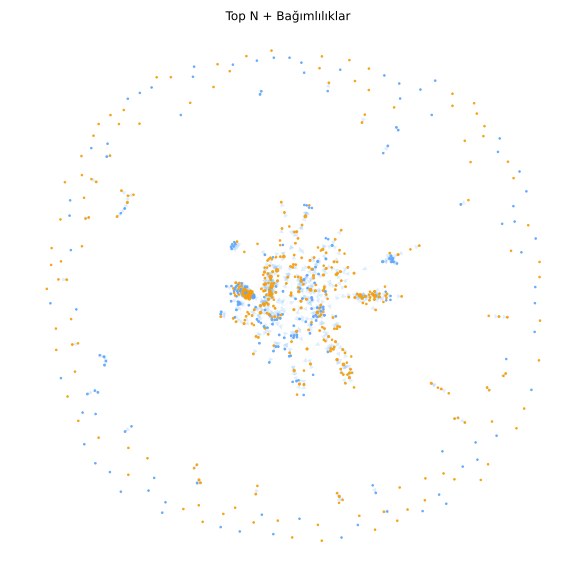
\includegraphics[width=\linewidth]{network_full_topN.png}
\caption{Top 1000 paket ağının görselleştirmesi. Yoğun bölgeler alt kümeleri işaret etmektedir.}
\label{fig:network}
\end{figure}

\begin{figure}[H]
\centering
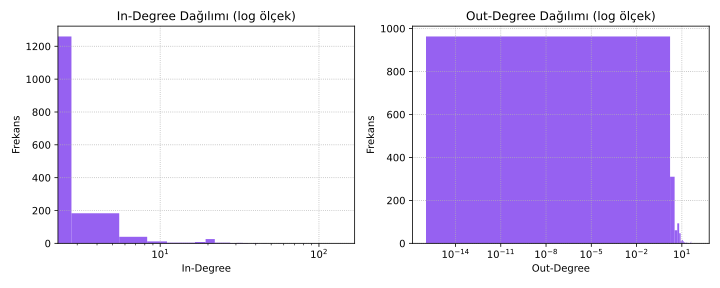
\includegraphics[width=\linewidth]{degree_histograms.png}
\caption{In-degree ve out-degree histogramları. Dağılımın ağır kuyruklu yapısı görülmektedir.}
\label{fig:histograms}
\end{figure}

Şekil \ref{fig:network}'te ağ topolojisinin kümelenme yapısı görülmektedir. Şekil \ref{fig:histograms}'teki derece dağılımları, ağın ölçekten bağımsız (scale-free) yapısını göstermektedir. Düğümlerin çoğunluğu az sayıda bağlantıya sahipken, az sayıda düğüm yüksek bağlantı sayısına sahiptir. Bu bulgu, riskin belirli bir bölümde yoğunlaştığını işaret etmektedir.

\subsection{Merkeziyet İlişkileri}
\begin{figure}[H]
\centering
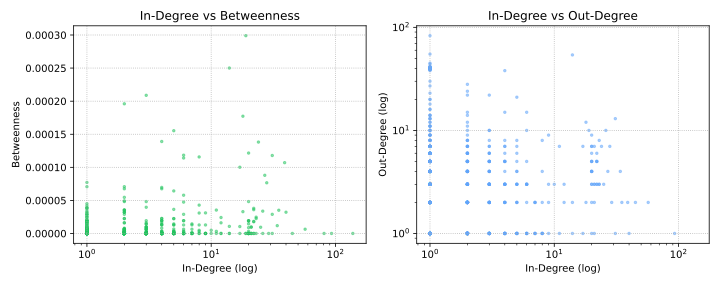
\includegraphics[width=\linewidth]{scatter_correlations.png}
\caption{Merkeziyet ölçüleri arasındaki korelasyonlar.}
\label{fig:scatter}
\end{figure}

Korelasyon matrisi (Şekil \ref{fig:scatter}), in-degree ile betweenness arasında asimetrik bir ilişki olduğunu göstermektedir. Yüksek popülariteye sahip olmayan bazı paketlerin köprü görevi gördüğü belirlenmiştir. Sadece indirme sayılarına odaklanan analizlerin yapısal riskleri tespit etmede yetersiz kalabileceği değerlendirilmektedir.

\subsection{Kritik Düğümlerin Analizi}
\begin{table}[H]
\centering
\caption{\textsc{Top 10 In-Degree}}
\label{tab:indegree}
\resizebox{\linewidth}{!}{%
\begin{tabular}{lrrrr}
\toprule
Paket & In-Degree & Out-Degree & Betweenness & TopN? \\
\midrule
@babel/helper-plugin-utils & 110 & 0 & 0.000000 & True \\
call-bound & 41 & 2 & 0.000283 & False \\
postcss-value-parser & 39 & 0 & 0.000000 & True \\
call-bind & 36 & 4 & 0.000000 & False \\
@types/node & 34 & 1 & 0.000067 & False \\
debug & 34 & 1 & 0.000100 & True \\
es-errors & 33 & 0 & 0.000000 & False \\
@babel/types & 32 & 2 & 0.000236 & True \\
define-properties & 29 & 3 & 0.000000 & False \\
chalk & 28 & 0 & 0.000000 & False \\
\bottomrule
\end{tabular}%
}
\end{table}

\begin{table}[H]
\centering
\caption{\textsc{Top 10 Out-Degree}}
\label{tab:outdegree}
\resizebox{\linewidth}{!}{%
\begin{tabular}{lrrrr}
\toprule
Paket & Out-Degree & In-Degree & Betweenness & TopN? \\
\midrule
@babel/preset-env & 70 & 3 & 0.000000 & True \\
postcss-preset-env & 67 & 1 & 0.000000 & True \\
es-abstract & 54 & 17 & 0.000000 & False \\
react-scripts & 48 & 0 & 0.000000 & True \\
workbox-build & 37 & 1 & 0.000000 & True \\
eslint & 34 & 1 & 0.000000 & True \\
cssnano-preset-default & 30 & 1 & 0.000000 & True \\
webpack-dev-server & 28 & 1 & 0.000000 & True \\
@jest/core & 28 & 2 & 0.000000 & True \\
express & 27 & 1 & 0.000000 & True \\
\bottomrule
\end{tabular}%
}
\end{table}

\begin{table}[H]
\centering
\caption{\textsc{Top 10 Betweenness}}
\label{tab:betweenness}
\resizebox{\linewidth}{!}{%
\begin{tabular}{lrrrr}
\toprule
Paket & Betweenness & In-Degree & Out-Degree & TopN? \\
\midrule
jest-circus & 0.001144 & 1 & 20 & False \\
@babel/core & 0.001112 & 12 & 15 & True \\
babel-jest & 0.001087 & 2 & 7 & True \\
jest-runner & 0.001000 & 2 & 22 & True \\
@babel/helper-create-class-features-plugin & 0.000798 & 10 & 7 & True \\
get-intrinsic & 0.000771 & 22 & 10 & True \\
jest-snapshot & 0.000549 & 6 & 21 & True \\
@babel/traverse & 0.000523 & 20 & 7 & True \\
babel-preset-current-node-syntax & 0.000499 & 2 & 15 & False \\
babel-plugin-istanbul & 0.000466 & 2 & 5 & True \\
\bottomrule
\end{tabular}%
}
\end{table}

Tablo \ref{tab:indegree}'deki yüksek in-degree değerine sahip paketler, sık kullanılan bileşenlerdir. Tablo \ref{tab:outdegree}'deki yüksek out-degree'li paketler geniş bir saldırı yüzeyi oluşturmaktadır. Tablo \ref{tab:betweenness}, ağ trafiğini yöneten paketleri göstermektedir. Örneğin, \texttt{jest-circus} paketi düşük in-degree (1) değerine sahip olmasına rağmen, yüksek betweenness değeriyle ağda kritik bir köprü rolü üstlenmektedir. Benzer şekilde \texttt{@babel/core}, hem popülerliği hem de stratejik konumuyla dikkat çekmektedir. Bu durum, risk analizinde tek bir metriğin yeterli olmadığını ve yapısal köprülerin tespitinin önemini kanıtlamaktadır.

\subsection{Bileşik Risk Skoru (BRS) Sıralaması}
\begin{figure}[H]
\centering
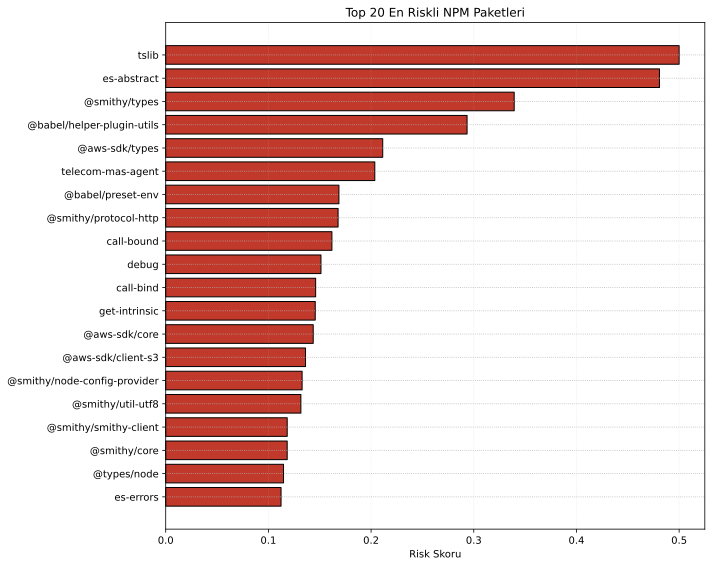
\includegraphics[width=\linewidth]{top20_risk_scores.png}
\caption{En yüksek Bileşik Risk Skoruna (BRS) sahip 20 paket.}
\label{fig:risk_scores}
\end{figure}

\begin{table}[H]
\centering
\caption{\textsc{Top 20 Bileşik Risk Skoru (BRS)}}
\label{tab:risk}
\resizebox{\linewidth}{!}{%
\begin{tabular}{lrrrrr}
\toprule
Paket & Risk & In-Degree & Out-Degree & Betweenness & TopN? \\
\midrule
@babel/helper-plugin-utils & 0.500000 & 110 & 0 & 0.000000 & True \\
@babel/core & 0.388827 & 12 & 15 & 0.001112 & True \\
jest-circus & 0.361688 & 1 & 20 & 0.001144 & False \\
jest-runner & 0.334157 & 2 & 22 & 0.001000 & True \\
get-intrinsic & 0.330606 & 22 & 10 & 0.000771 & True \\
babel-jest & 0.313975 & 2 & 7 & 0.001087 & True \\
@babel/helper-create-class-features-plugin & 0.274757 & 10 & 7 & 0.000798 & True \\
call-bound & 0.266206 & 41 & 2 & 0.000283 & False \\
@babel/traverse & 0.248118 & 20 & 7 & 0.000523 & True \\
es-abstract & 0.231558 & 17 & 54 & 0.000000 & False \\
jest-snapshot & 0.231168 & 6 & 21 & 0.000549 & True \\
@babel/preset-env & 0.213636 & 3 & 70 & 0.000000 & True \\
@babel/types & 0.212942 & 32 & 2 & 0.000236 & True \\
postcss-preset-env & 0.195974 & 1 & 67 & 0.000000 & True \\
@jest/types & 0.193414 & 26 & 7 & 0.000211 & True \\
debug & 0.183565 & 34 & 1 & 0.000100 & True \\
babel-preset-current-node-syntax & 0.182762 & 2 & 15 & 0.000499 & False \\
postcss-value-parser & 0.177273 & 39 & 0 & 0.000000 & True \\
call-bind & 0.175065 & 36 & 4 & 0.000000 & False \\
@types/node & 0.174844 & 34 & 1 & 0.000067 & False \\
\bottomrule
\end{tabular}%
}
\end{table}
BRS modeli; popülerlik, saldırı yüzeyi ve stratejik konumu birleştirmektedir. Şekil \ref{fig:risk_scores} ve Tablo \ref{tab:risk}'te görüldüğü üzere, hem popülerliği hem de ağ konumu nedeniyle belirli paketler üst sıralarda yer almaktadır. Sıralama, güvenlik denetimlerinde önceliklendirilecek paketleri göstermektedir.

\subsection{Sistemik Etki ve Kaskad Analizi}
\begin{figure}[H]
\centering
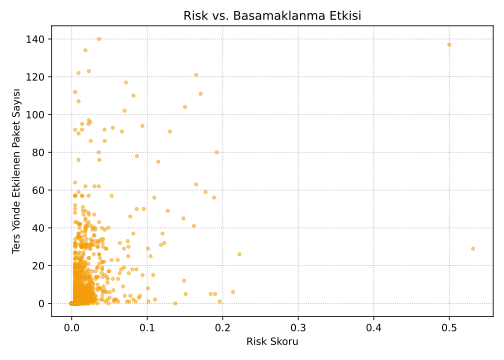
\includegraphics[width=\linewidth]{risk_vs_cascade.png}
\caption{BRS ile kaskad etki (erişilebilirlik) arasındaki ilişki.}
\label{fig:cascade}
\end{figure}

\begin{figure}[H]
\centering
\includegraphics[width=\linewidth]{top20_cascade_impact.png}
\caption{İlk 20 paketin çıkarılmasının LCC ve erişilebilirlik üzerindeki etkisi.}
\label{fig:impact}
\end{figure}
Simülasyon sonuçları BRS modelini desteklemektedir. Şekil \ref{fig:impact}'te, yüksek BRS skorlu paketlerin çıkarılmasının LCC boyutunda düşüşe neden olduğu görülmektedir. BRS skoru ile kaskad etki arasındaki korelasyon (Şekil \ref{fig:cascade}), metriğin risk öngörüsündeki başarısını göstermektedir.

\section{Tartışma ve Sonuç}
Bu çalışmada, literatürdeki betimsel analizlerin ötesine geçilerek, NPM ekosistemindeki yapısal riskleri ölçülebilir bir değere dönüştüren \textbf{Bileşik Risk Skoru (BRS)} modeli sunulmuştur. Giriş bölümünde belirtilen "operasyonel önceliklendirme" eksikliği, elde edilen BRS sıralaması ile giderilmiştir. Analizler, ağın güvenliğinin sadece popüler paketlere değil, \texttt{jest-circus} veya \texttt{@babel/core} gibi altyapısal köprü paketlere de bağlı olduğunu göstermiştir. Elde edilen bulgular, Zimmermann ve arkadaşlarının \cite{zimmermann2019smallworld} belirttikleri "küçük dünya" ağ yapısını doğrulamakta; ancak riskin sadece popüler paketlerde değil, köprü (bridge) niteliğindeki ara katman paketlerinde de yoğunlaştığını ortaya koyarak literatürü genişletmektedir.

\subsection{Çalışmanın Kısıtları}
Analiz, \texttt{package.json} dosyalarında tanımlı statik bağımlılıklar ile sınırlandırılmıştır. Çalışma zamanında (runtime) dinamik olarak yüklenen paketler veya geliştirici hesaplarının güvenilirliği (reputation) bu aşamada kapsam dışı bırakılmıştır. Ayrıca analiz, anlık bir kesit (snapshot) üzerinden yapılmış olup, ağın zamansal evrimini içermemektedir. Benzer şekilde, lisans uyumluluğu gibi yasal riskler \cite{ahlstrom2025licensing} de bu çalışmanın kapsamı dışındadır.

\subsection{Öneriler}
Bulgular doğrultusunda aşağıdaki öneriler geliştirilmiştir:
\begin{itemize}
    \item \textbf{Önceliklendirme:} Güvenlik taramalarında kaynakların BRS skoru yüksek paketlere yönlendirilmesi.
    \item \textbf{Politika Geliştirme:} Güvenlik protokollerinin \cite{torres2020intoto} ve SBOM uygulamalarının \cite{yu2024sbom} kritik düğümlere uygulanması.
    \item \textbf{Farkındalık:} Paket sahiplerinin risk skorları hakkında bilgilendirilmesi.
\end{itemize}

Gelecek çalışmalarda modelin geliştirici ağlarını kapsayacak şekilde genişletilmesi önerilmektedir.

\section{Yen{\footnotesize İ}den Üret{\footnotesize İ}leb{\footnotesize İ}rl{\footnotesize İ}k}
Çalışmanın tekrarlanabilirliği için kaynak kodlar ve veri setleri paylaşılmıştır:
\begin{itemize}
  \item \textbf{Analiz Kodları:} \texttt{analysis/analysis.ipynb} (Python 3, NetworkX, pandas).
  \item \textbf{Veri Çıktıları:} Tüm ara sonuçlar ve metrikler \texttt{results/} dizininde CSV/JSON formatında sunulmuştur.
\end{itemize}

% APA-style bibliography 
\begin{thebibliography}{30}

\bibitem{lit1} E. Wyss, ``A new frontier for software security: Diving deep into npm,'' 2025.

\bibitem{lit7} M. Wang, P. Wu, and Q. Luo, ``Construction of software supply chain threat portrait based on chain perspective,'' 2023.

\bibitem{lit8} C. Liu et al., ``Demystifying vulnerability propagation via dependency trees in npm,'' in \textit{ICSE}, 2022.

\bibitem{lit18} A. Zerouali et al., ``On the impact of security vulnerabilities in the npm and RubyGems dependency networks,'' 2022.

\bibitem{lit5} I. Rahman et al., ``Characterizing dependency update practice of NPM, PyPI and Cargo packages,'' 2024.

\bibitem{lit22} F. R. Cogo, ``Studying dependency maintenance practices through mining NPM,'' 2020.

\bibitem{lit10} A. J. Jafari et al., ``Dependency practices for vulnerability mitigation,'' 2023.

\bibitem{lit20} M. Zimmermann et al., ``Small world with high risks: Security threats in npm,'' in \textit{USENIX Sec.}, 2019.

\bibitem{lit16} A. Hafner, A. Mur, and J. Bernard, ``Node package manager's dependency network robustness,'' 2021.

\bibitem{lit25} E.-R. Oldnall, ``The web of dependencies: A complex network analysis of the NPM,'' 2017.

\bibitem{lit2} P. Jaisri, B. Reid, and R. G. Kula, ``A preliminary study on self-contained libraries in the NPM ecosystem,'' 2024.

\bibitem{lit6} T. G. Hastings, ``Combating source poisoning and next-generation software supply chain attacks,'' 2024.

\bibitem{lit30} M. Shcherbakov, P. Moosbrugger, and M. Balliu, ``Unveiling the invisible: Prototype pollution gadgets via dynamic taint,'' 2021.

\bibitem{lit12} D. Y. K. Yip, ``Empirical study on dependency-based attacks in Node.js,'' 2022.

\bibitem{lit4} M. Ohm et al., ``Backstabber's knife collection: A review of open source software supply chain attacks,'' in \textit{DIMVA}, 2020.

\bibitem{lit24} P. Ladisa et al., ``The hitchhiker's guide to malicious third-party dependencies,'' in \textit{IEEE S\&P}, 2023.

\bibitem{lit28} R. Duan et al., ``Towards measuring supply chain attacks on package managers,'' in \textit{NDSS}, 2020.

\bibitem{lit19} A. Sejfia and M. Schafer, ``Practical automated detection of malicious npm packages (Amalfi),'' in \textit{ICSE}, 2022.

\bibitem{lit29} X. Zheng et al., ``Towards robust detection of OSS supply chain poisoning (OSCAR),'' 2024.

\bibitem{lit15} S. Halder et al., ``Malicious package detection using metadata information,'' 2024.

\bibitem{lit14} J. Zhang et al., ``Malicious package detection in NPM and PyPI using a single model of malicious behavior sequence,'' 2023.

\bibitem{lit17} P. Ladisa et al., ``On the feasibility of cross-language detection of malicious packages in npm and PyPI,'' 2023.

\bibitem{lit11} M. L. P. Correia, ``Detection of software supply chain attacks in code repositories,'' 2022.

\bibitem{lit23} M. Ohm et al., ``Supporting detection via unsupervised signature generation (ACME),'' 2021.

\bibitem{lit13} S. Torres-Arias, ``In-toto: Practical software supply chain security,'' in \textit{USENIX Sec.}, 2020.

\bibitem{lit3} S. Yu, ``Accurate and efficient SBOM generation for software supply chain security,'' 2024.

\bibitem{lit9} H. E. Ahlstrom, ``Dependency analysis for software licensing and security,'' 2025.

\bibitem{lit21} T. R. Schorlemmer, ``Software supply chain security: Attacks, defenses, and signing adoption,'' 2024.

\bibitem{lit26} N. Imtiaz, ``Toward secure use of open source dependencies,'' 2023.

\bibitem{lit27} S. Vaidya, ``Towards ensuring integrity and authenticity of software repositories,'' 2022.

\end{thebibliography}


\end{document}